\documentclass[12pt]{beamer}
\author{Yan Wang}
\title{Paper Reading Seminar}
\subtitle{}
\usetheme{Malmoe}
\setbeamertemplate{navigation symbols}{}
\newcommand*\oldmacro{}%
\let\oldmacro\insertshorttitle%
\renewcommand*\insertshorttitle{%
\oldmacro\hfill%
\insertframenumber\,/\,\inserttotalframenumber}

\begin{document}

\begin{frame}[plain]
    \titlepage
\end{frame}

\begin{frame}{Combining Randomization and Discrimination for Fine-Grained Image Categorization}
    \begin{itemize}
        \item Motivation
        \medskip
        { 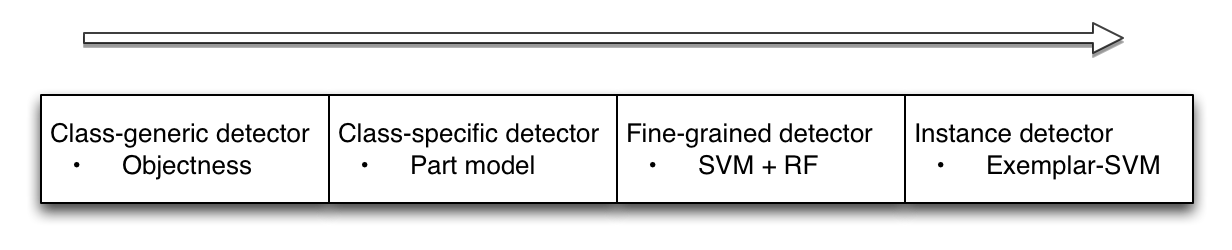
\includegraphics[width=0.8\textwidth]{motivation.png} } 
        \begin{itemize}
            \item Fine-grained image categorization
            \item Bird species
            \item Human activity classification
        \end{itemize}
        \item Intuition
        \begin{itemize}
            \item Dense sampling $\Rightarrow$ patches
            \item Correlation among patches
            \item Random forest + SVM
        \end{itemize}
    \end{itemize}
\end{frame}

\begin{frame}{Approach}
    \begin{itemize}
        \item Dense sampling \\
        \medskip
        { 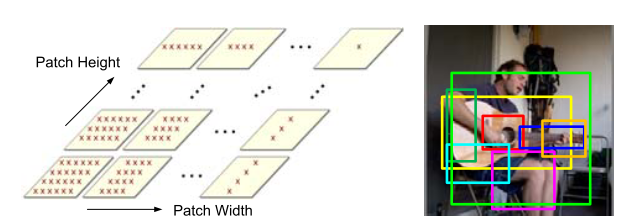
\includegraphics[width=0.6\textwidth]{fffig2.png} } \\
        \item Feature
        \begin{itemize}
            \item Single patch: BoW
            \item Patch pair: concatenation/intersection/absolute of difference of BoW histogram
        \end{itemize} 
    \end{itemize}
\end{frame}

\begin{frame}{Approach}
    \begin{itemize}
        \item Random forest + SVM \\
        \medskip
        { 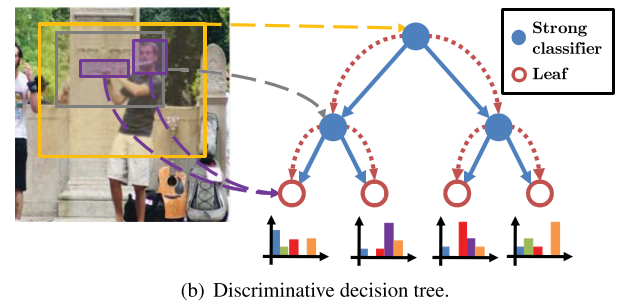
\includegraphics[width=0.7\textwidth]{fffig3.png} }
        \begin{itemize}
            \item Randomly select patches (or patch pairs) + SVM
            \item Train random forest with information gain
            \item Use ``ancestor'' features
            \item Q: invariance?
        \end{itemize}
    \end{itemize}
\end{frame}

\begin{frame}{Application}
    \begin{itemize}
        \item Heatmap \\
        \medskip
        { 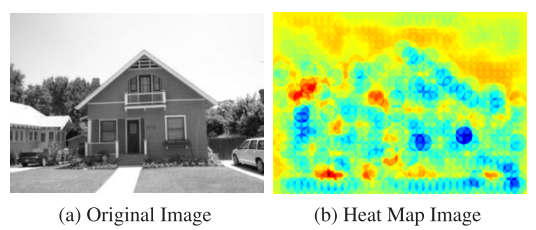
\includegraphics[width=0.7\textwidth]{fig1.png} }
        \item Frequency a region picked up by the random forest
        \item Visualize from a classifier's perspective
    \end{itemize}
\end{frame}
\begin{frame}{Measuring the objectness of image windows}
    \begin{itemize}
        \item Motivation
        \medskip
        { 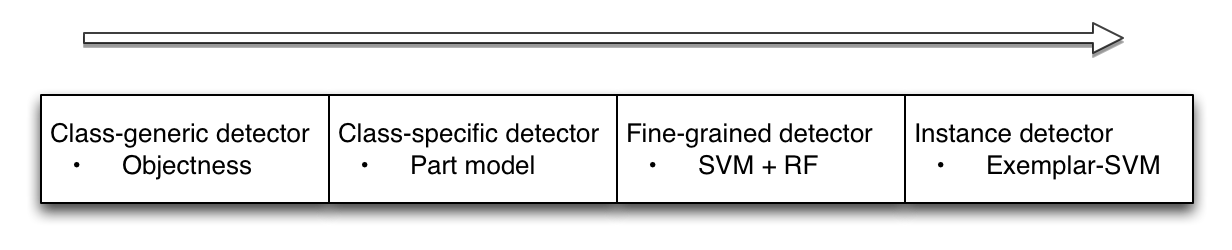
\includegraphics[width=0.8\textwidth]{motivation.png} } 
        \begin{itemize}
            \item Hand-crafted model $\Rightarrow$ different from conventional ``detectors''
        \end{itemize}
        \item Applications
        \begin{itemize}
            \item Preprocessing for detection
            \item Visualization of classifier
            \item Foreground/background separation?
        \end{itemize}
    \end{itemize}
\end{frame}

\begin{frame}{Approach}
    \begin{itemize}
        \item Intuition: an object should have...
        \begin{itemize}
            \item A well defined closed boundary in space
            \item A different appearance from its surroundings
            \item Sometimes unique within the image (salient)
        \end{itemize}
        \item Bayesian fusion of the cues
    \end{itemize}
\end{frame}

\begin{frame}{Approach}
    \begin{itemize}
        \item Multi-scale saliency
        \begin{itemize}
            \item Spectral residual of FFT in multiple scales
            \item Measure the uniqueness of the window within the image
        \end{itemize}
        \medskip
        { 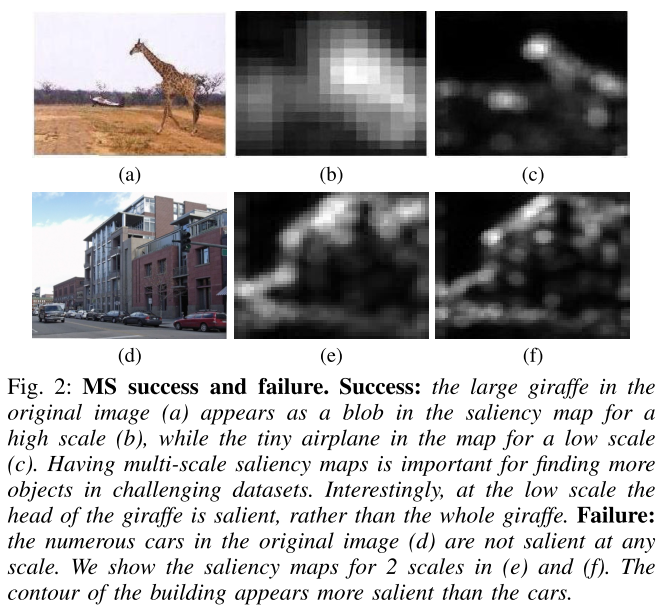
\includegraphics[width=0.6\textwidth]{fig2.png} } 
    \end{itemize}
\end{frame}

\begin{frame}{Approach}
    \begin{itemize}
        \item Color contrast
        \begin{itemize}
            \item Dissimilarity of a window to its immediate surrounding area
            \item Chi-square distance between LAB histogram
            \item Scores a whole window as whether it contains an entire project
        \end{itemize}
        \medskip
        { 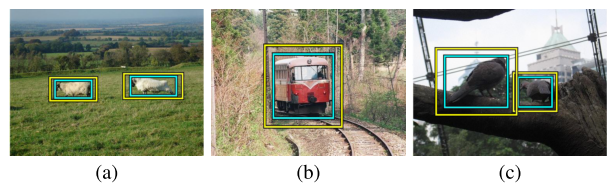
\includegraphics[width=0.8\textwidth]{fig3.png} } 
    \end{itemize}
\end{frame}

\begin{frame}{Approach}
    \begin{itemize}
        \item Edge Density
        \begin{itemize}
            \item Canny detector in the inner ring. Normalized with perimeter
            \item Captures the closed boundary characteristic of objects
        \end{itemize}
        \medskip
        { 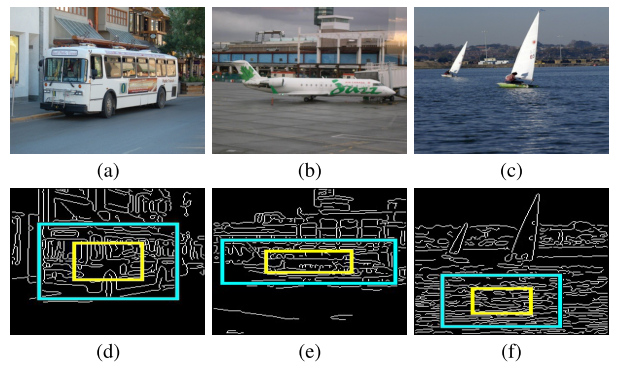
\includegraphics[width=0.6\textwidth]{fig4.png} } 
    \end{itemize}
\end{frame}

\begin{frame}{Approach}
    \begin{itemize}
        \item Superpixel Straddling
        \begin{itemize}
            \item Superpixels shouldn't cross the bondary
            \item Rely on over-segmentation
        \end{itemize}
        \medskip
        { 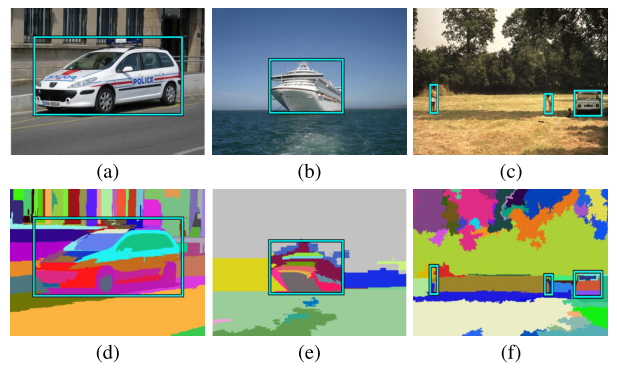
\includegraphics[width=0.6\textwidth]{fig6.png} } 
    \end{itemize}
\end{frame}

\begin{frame}{Approach}
    \begin{itemize}
        \item Spatial priori
        \begin{itemize}
            \item Location and size
            \item Kernel density estimation from training data
        \end{itemize}
        \item Bayesian fusion
        \[p(\text{obj}|C) = \frac{p(C|\text{obj})p(\text{obj})}{p(C)}\]
    \end{itemize}
\end{frame}

\end{document}

